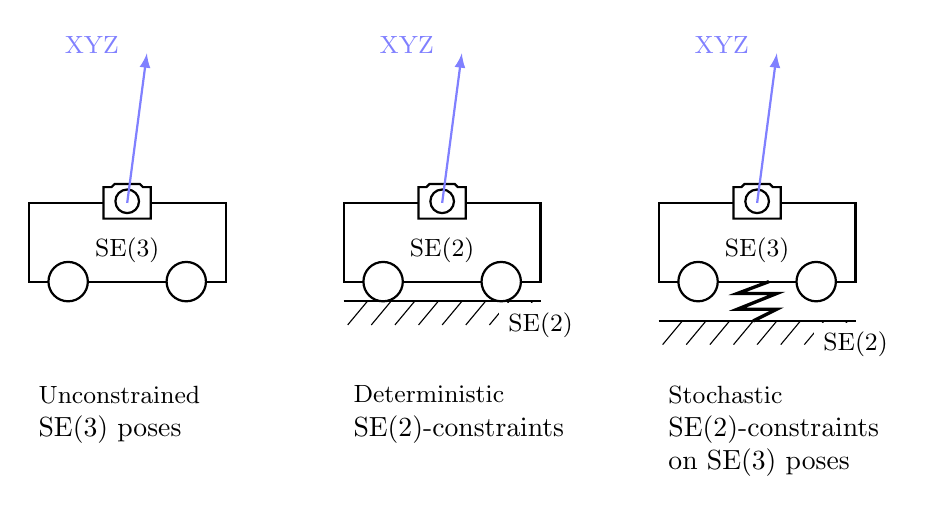
\begin{tikzpicture}[>=latex,scale=1.0,
  ]

  \def\cameraicon#1#2{
    \begin{scope}[shift={#1}, rotate=#2]
      \draw[thick,fill=white] (-0.3,-0.2) -- (0.3,-0.2) -- (0.3,0.2) -- (0.2,0.2) --
      (0.16,0.24) -- (-0.16,0.24)--(-0.2,0.2)--(-0.3,0.2)--cycle;
      \draw[thick,fill=white] (0,0.02) circle [radius=0.15];
    \end{scope}
  }
  % \draw[gray!50,step=0.5] (0,0) grid (12,6);
  \foreach \x in {0.5,4.5,8.5}
  {
    \draw[thick] (\x,2) rectangle (\x+2.5,3);
    \draw[thick,fill=white] (\x+0.5,2) circle [radius=0.25];
    \draw[thick,fill=white] (\x+2,2) circle [radius=0.25];
    \draw[blue!50] (\x+1.5,5) node {\Large $\bigstar$};
    \draw[blue!50] (\x+0.8,5) node {\small XYZ};
    \cameraicon{(\x+1.25,3)}{0}
    \draw[blue!50,thick,->] (\x+1.25,3) -- (\x+1.5,4.9);
  }
  \foreach \x in {1,2,3,4,5,6,7,8}
  {
    \draw (4.5+\x*0.30,1.75) -- +(-0.25,-0.3);
    \draw[xshift=4cm,yshift=-0.25cm] (4.5+\x*0.30,1.75) -- +(-0.25,-0.3);
  }
  \draw[] (1.75,2.4) node {\small SE(3)};
  \draw[] (5.75,2.4) node {\small SE(2)};
  \draw[] (9.75,2.4) node {\small SE(3)};
  \draw[yshift=0.25cm] (7,1.2) node[fill=white] {\small SE(2)};
  \draw[xshift=4cm] (7,1.2) node[fill=white] {\small SE(2)};
  \draw[thick] (4.5,1.75) -- (7,1.75);
  \draw[thick,xshift=4cm,yshift=-0.25cm] (4.5,1.75) -- (7,1.75);
  \draw[very thick] (9.7,1.5) -- (10,1.65) -- (9.5,1.65) -- (10,1.85) -- (9.5,1.85) --(9.9,2);

  \draw (0.5,0.8) node[below right,align=left] {\small Unconstrained\\ SE(3) poses};
  \draw[xshift=4cm] (0.5,0.8) node[below right,align=left] {\small Deterministic\\ SE(2)-constraints};
  \draw[xshift=8cm] (0.5,0.8) node[below right,align=left] {\small Stochastic\\ SE(2)-constraints\\ on SE(3) poses};

\end{tikzpicture}
